\documentclass[aspectratio=169,xcolor={table, dvipsnames}]{beamer}

\usepackage{svg}
\usepackage{graphicx}
\usepackage{tabularx}
\usepackage{booktabs}
\usepackage{tikz}
\usepackage{standalone}
\usepackage{caption}
\usepackage{subcaption}
\usepackage{xcolor}
\usepackage{hyperref}

\usepackage[backend=biber]{biblatex}

\addbibresource{2024_ad-fidelity.bib}

\usetikzlibrary{positioning, shadows, fit, backgrounds, overlay-beamer-styles, shapes.arrows}

% make references tiny, so they don't take up much slides
\renewcommand*{\bibfont}{\tiny}

% modern minimalist latex theme
\usetheme{metropolis}

% fill blocks with background color
\metroset{block=fill}

% footer
\setbeamertemplate{frame footer}{\href{https://github.com/chillerb}{\insertshortauthor}\hfill\insertshorttitle}

%\setbeamertemplate{frame footer}{\insertshortauthor~(\insertshortinstitute)}


\renewcommand{\emph}[1]{\textbf{#1}}

\title[Fidelity of Explanations for AD Classification from MRI]{Evaluating the Fidelity of Explanations for Convolutional Neural Networks in Alzheimer’s Disease Detection}

\author[Hiller]{Bjarne C. Hiller}
\date{2025-03-09}
\institute[Uni Rostock]{University of Rostock}

%\logo{
\includegraphics[height=0.5cm]{logos/logo-uni-hro}}

\titlegraphic{
    \href{https://vac.uni-rostock.de/}{
\includegraphics[height=1cm]{logos/logo-vac}}\hfill
    \href{https://www.uni-rostock.de/}{
\includegraphics[height=1cm]{logos/logo-uni-hro}}\hfill
	\href{https://www.dzne.de/}{
\includegraphics[height=1cm]{logos/logo-dzne}}
}

\begin{document}

\maketitle

% \begin{frame}{Agenda}
% 	\tableofcontents
% \end{frame}


% \begin{frame}{Deep Learning for Medical Image processing}
% 	% introduce deep learning and XAI
% 	% - want to analyse MRI from AD subjects
% 	% - Deep Learning powerful for image processing, expert level performance
% 	% - however, Black Box systems
% 	% - Can we trust prediction?
% \end{frame}

\begin{frame}{Data and Network}
	\centering
	\begin{block}{Data and Preprocessing}
		\vfill
		\begin{itemize}
			\item $N=443$ ($AD = 189$, $CN=254$) T1-weighted MRI from ADNI database
			\item Skull Stripping, Gray-matter segmentation, Non-linear registration (MNI)
		\end{itemize}
	\end{block}
	\visible<2->{
		\begin{tikzpicture}
			\node [draw, rectangle, fill=white, drop shadow, inner sep=0] (cnn) {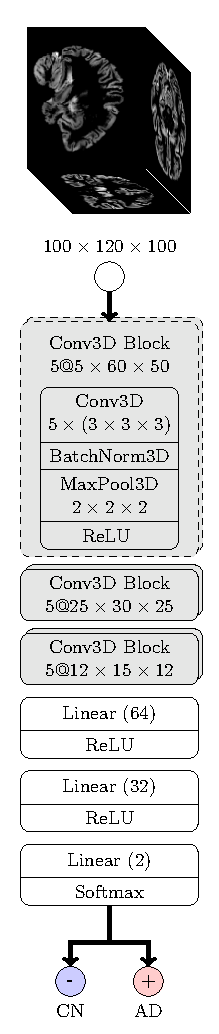
\includegraphics[angle=90, width=\textwidth]{tikz/standalone/cnn.tikz/cnn.pdf}};
		\end{tikzpicture}
	}
	\visible<3->{
		\emph{But can the model be trusted?}
	}


	%	\begin{columns}[T]
	%		\begin{column}{0.5\textwidth}
	%			\begin{block}{ADNI Data and Preprocessing}
	%				\vfill
	%				\begin{itemize}
	%					\item $N=443$ ($AD = 189$) T1 MRI
	%					\item Gray-matter segmentation
	%					\item Non-linear registration to MNI
	%				\end{itemize}
	%			\end{block}
	%		\end{column}\hfill
	%		\begin{column}{0.5\textwidth}
	%			\begin{block}{Problem}
	%				Can the model be trusted?
	%				\vfill
	%			\end{block}
	%		\end{column}
	%	\end{columns}
\end{frame}

\begin{frame}{Attribution Maps: What did the network look at?}
	\begin{figure}
		\centering
		\begin{tikzpicture}
			\node [draw, rectangle, fill=white, drop shadow, inner sep=0] (cnn) {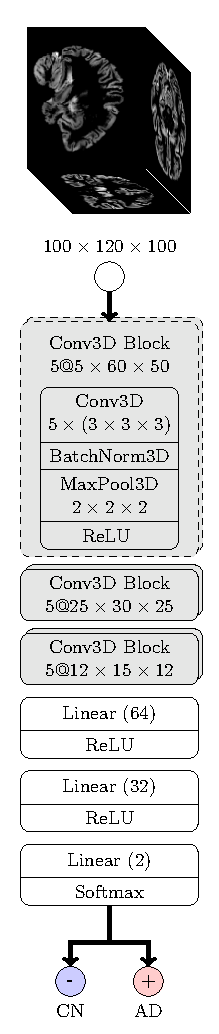
\includegraphics[angle=90, width=\textwidth]{tikz/standalone/cnn.tikz/cnn.pdf}};
			\visible<2->{
				\node[draw=red, ultra thick, rectangle, anchor=east, minimum width=1.5cm, minimum height=3cm] (outbox) at (cnn.east) {};
				%\draw[draw=red, ->, ultra thick] (outbox.south) -- ++ (0, -1) --++ (-10,0) node[midway, below] {\emph{Relevance Propagation}} node[at end] (backprop){};
				\node[below=0.5cm of cnn.south west, anchor=north west, draw, rectangle, inner sep=0, drop shadow, label=below:relevance map] (attribution) {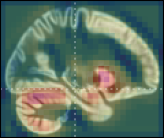
\includegraphics[height=2cm]{figures/grad-cam-map.png}};
				\draw[draw=red, ->, ultra thick] (outbox.south) |- (attribution.east) node[midway, below, anchor=north east] {\emph{Propagation of Relevance}};
			}
		\end{tikzpicture}
		%\caption*{Attribution of change in model output to change in model input.}\label{fig:attribution}
	\end{figure}
\end{frame}

\begin{frame}[plain]{Why should I care?}
	\centering
	\begin{figure}
		\begin{subfigure}[b]{0.3\textwidth}
			\centering
			\begin{tikzpicture}
				\node[inner sep=0, draw, rectangle, drop shadow] (tinauer) {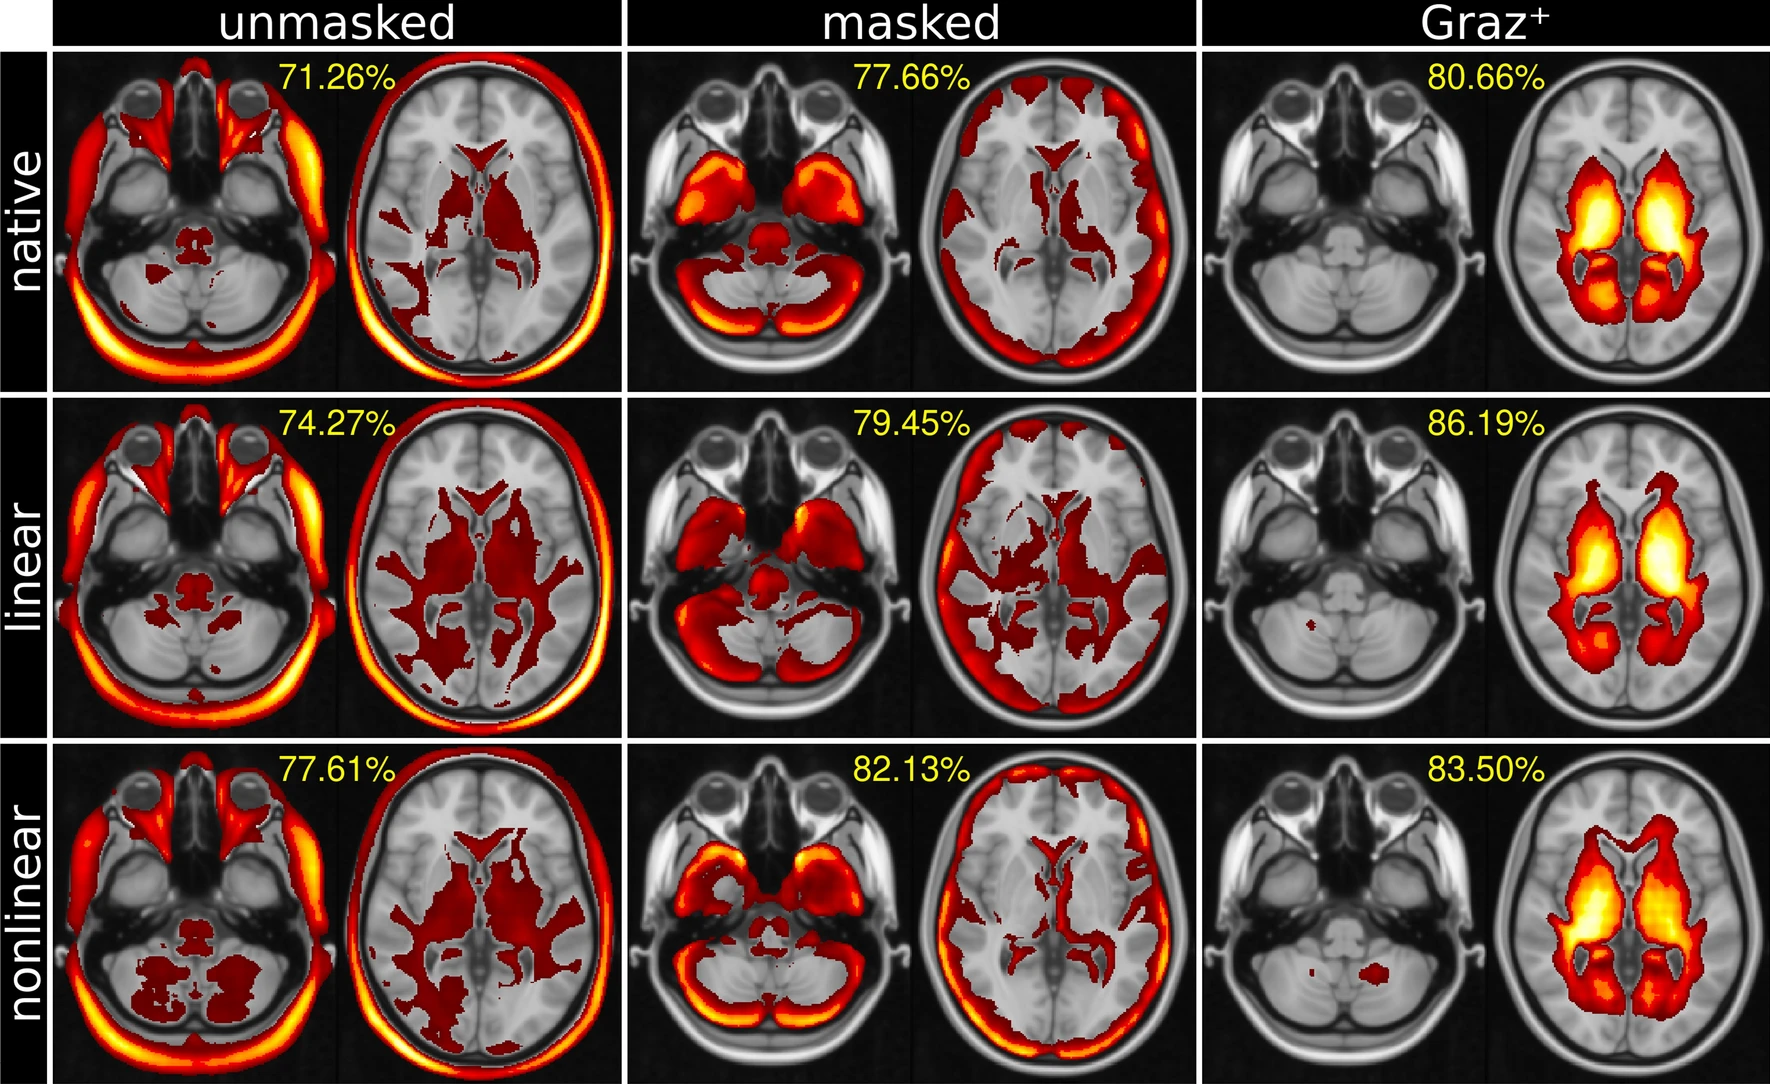
\includegraphics[height=5cm, trim={0 0 1150px 0}, clip]{figures/tinauer_2022.png}};
				\begin{scope}[overlay, visible on=<2->]
					\draw[<-, red, ultra thick] (tinauer.east) -- ++ (0.5,0) node (pointerstart) {};
					\draw[->, red, ultra thick] (pointerstart.center) |- ++ (-0.5,1.5);
					\draw[->, red, ultra thick] (pointerstart.center) |- ++ (-0.5,-1.7);
				\end{scope}
			\end{tikzpicture}
			\caption{From: \citeauthor{tinauer_interpretable_2022}~\cite{tinauer_interpretable_2022}}\label{fig:tinauer}
		\end{subfigure}\hfill
		\begin{subfigure}[b]{0.7\textwidth}
			\begin{tikzpicture}
				\node[inner sep=0, draw, rectangle, drop shadow] (tinauer) {
					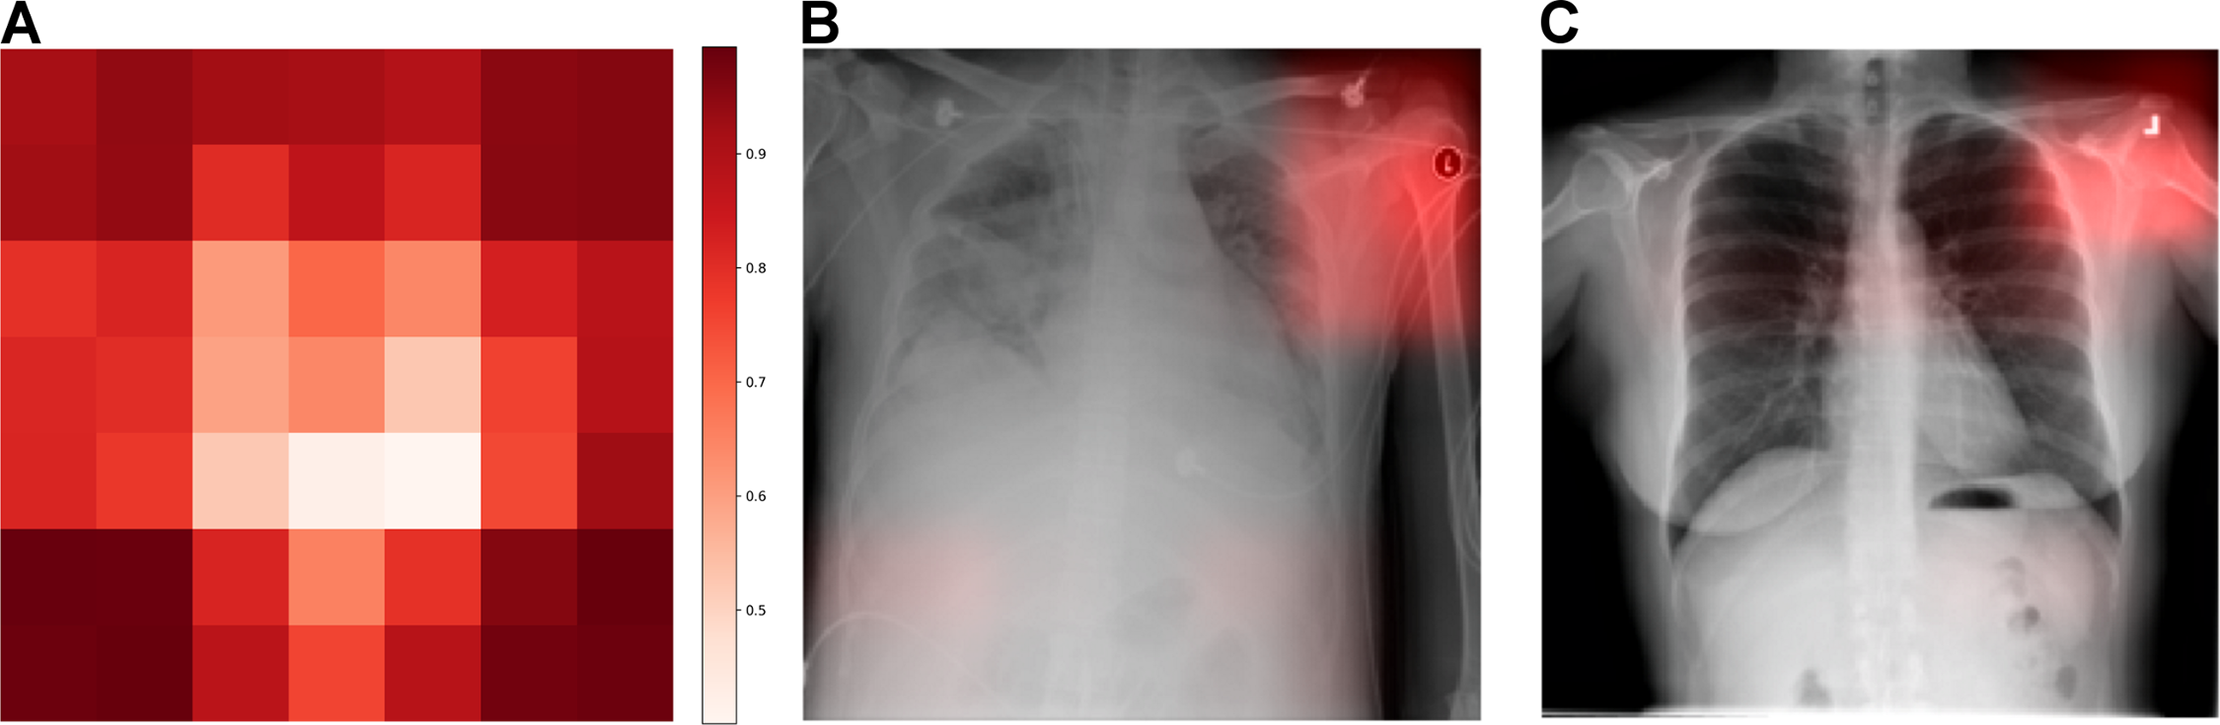
\includegraphics[height=5cm, trim={190px 0 0 0}, clip]{figures/zech_2018.png}
				};
				\begin{scope}[overlay, visible on=<3->]
					\node[red, ultra thick, circle, draw, minimum width=2cm] at (-0.9,1.1) {};
					\node[red, ultra thick, circle, draw, minimum width=2cm] at (4.5,1.5) {};
				\end{scope}
			\end{tikzpicture}
			\caption{From: \citeauthor{zech_variable_2018}~\cite{zech_variable_2018}}\label{fig:zech}
		\end{subfigure}
		\caption*{Attribution maps can reveal \emph{shortcut learning}:  Neural Networks can use features outside of the brain parenchyma (\subref{fig:tinauer}) or X-ray side marker tokens (\subref{fig:zech}) for classification.}
	\end{figure}

\end{frame}

\begin{frame}[plain]
	%{eXplainable AI and Feature Attribution Methods}
	% - explain overall principle of feature attribution methods
	% - plethora of feature attribution methods
	% - Can we trust *explanation*?
	% - "Not sure, if model is broken, or explanation is wrong"
	\begin{figure}
		\centering
		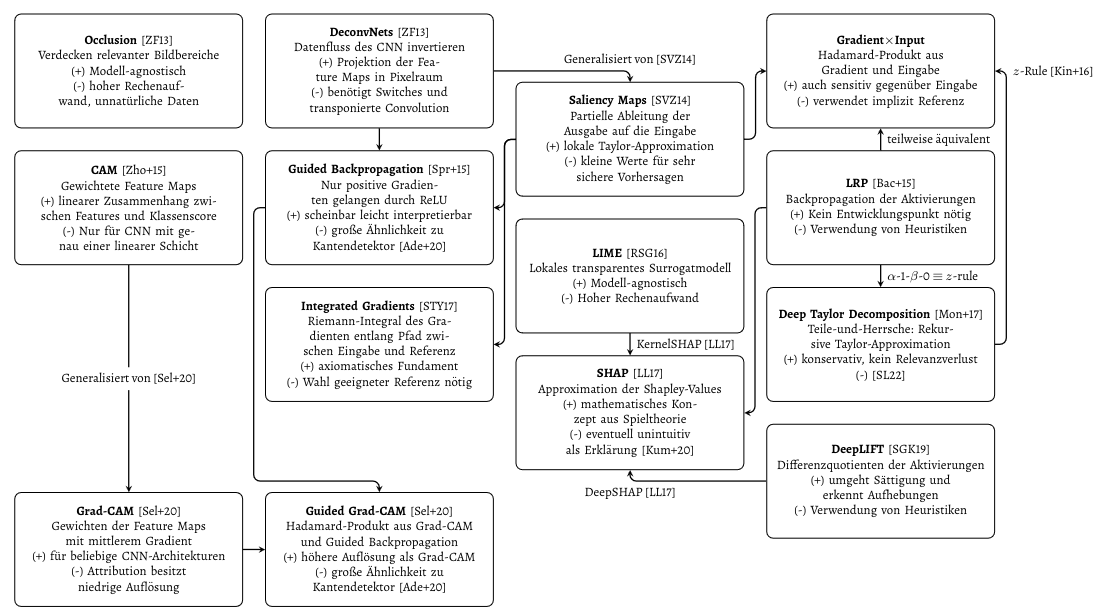
\includegraphics[width=0.9\textwidth]{figures/overview.png}
		\caption*{Popular feature attribution methods for Deep Neural Networks and their Relationships}
	\end{figure}
\end{frame}

\begin{frame}[plain]
	\centering
	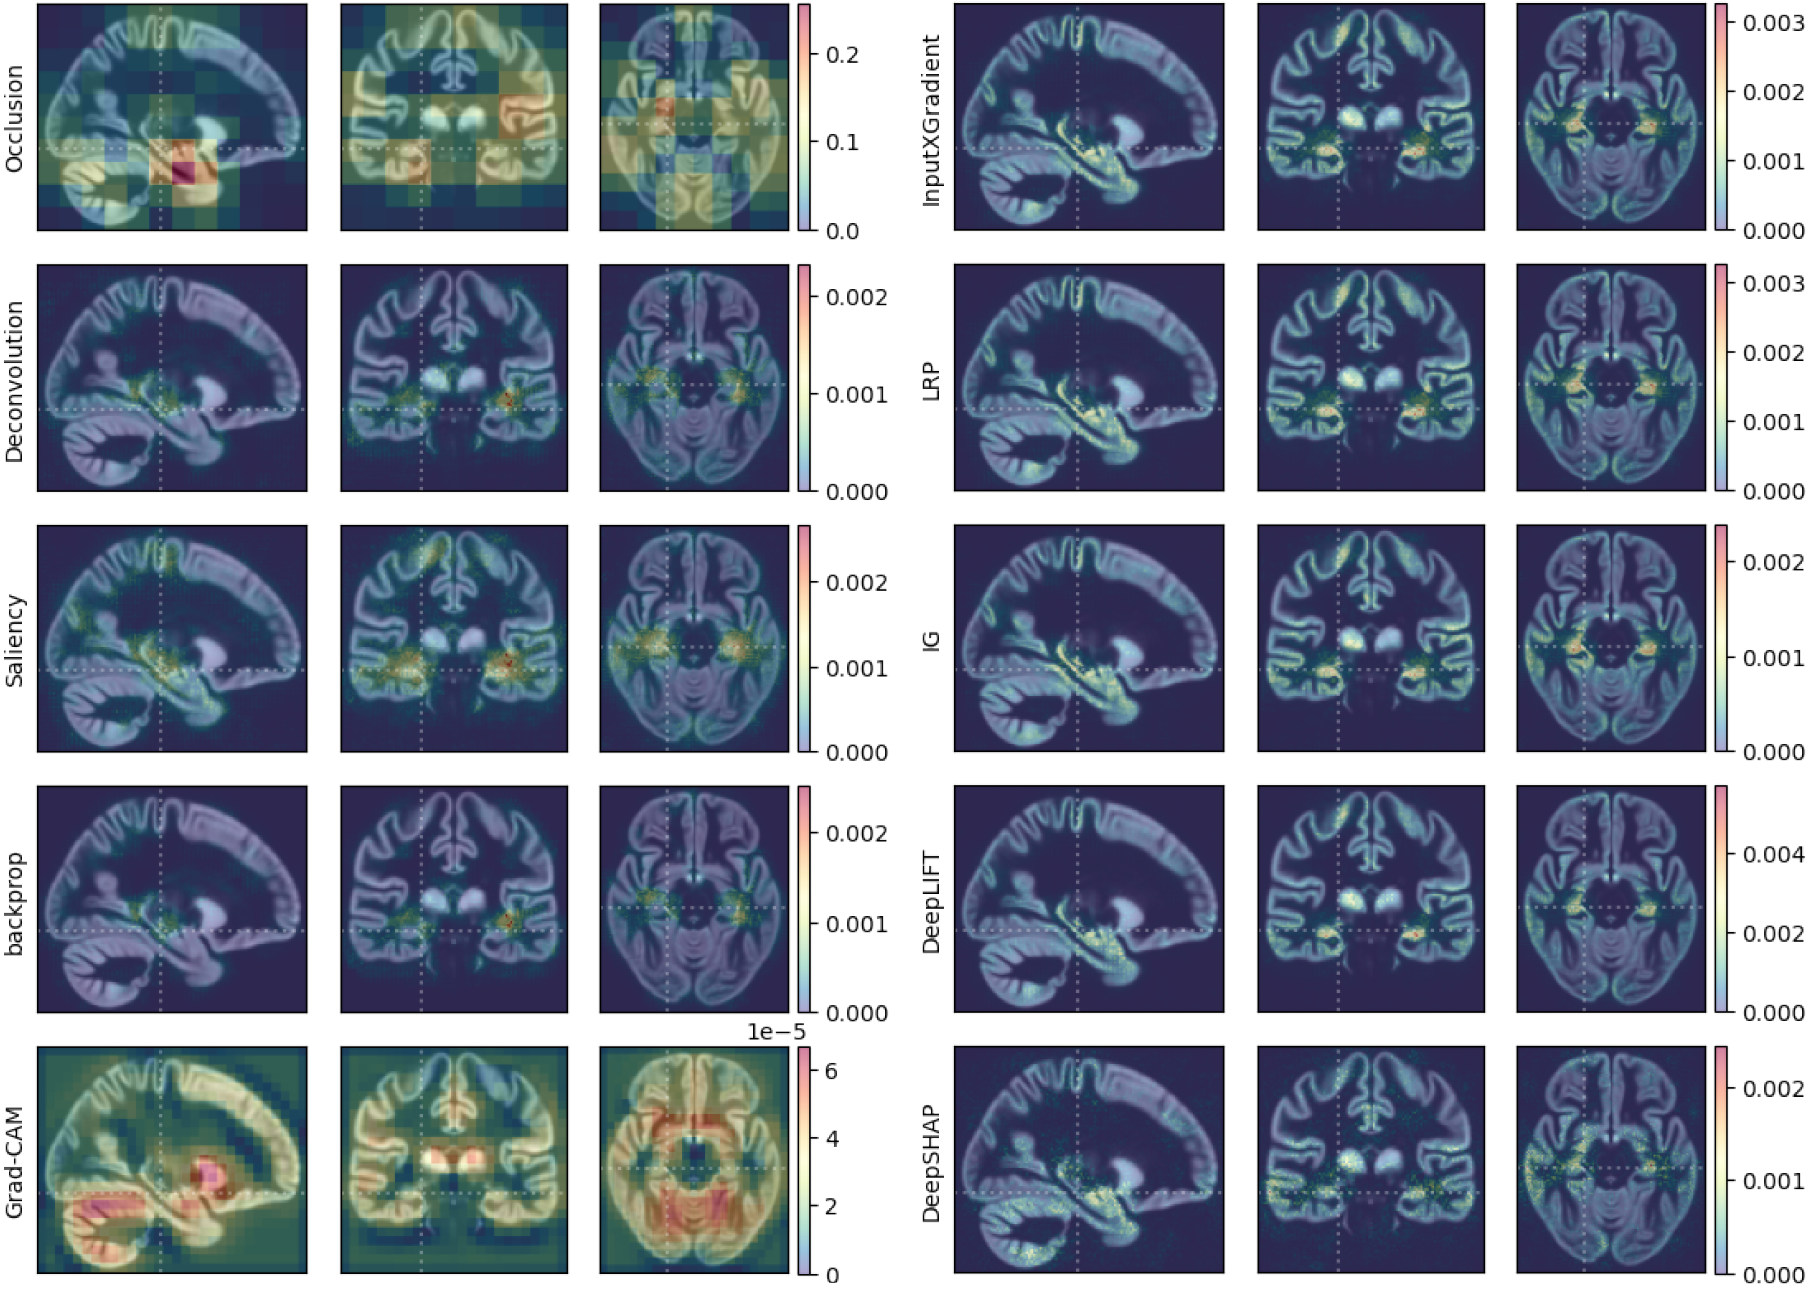
\includegraphics[width=0.85\textwidth]{figures/3672-relevance-maps.png}
\end{frame}

\begin{frame}{Total Relevance per ROI}
	\begin{table}
	\centering
	\footnotesize
	\rowcolors{2}{white}{gray!25}
	\begin{tabularx}{\textwidth}{lXXXX}
		\toprule
		    & Occlusion               & IG                    & DeepLIFT              & DeepSHAP        \\
		\midrule
		1.  & Precuneus\_L            & Temporal\_Mid\_L      & Temporal\_Mid\_L      & Calcarine\_L    \\
		2.  & Precuneus\_R            & Temporal\_Mid\_R      & Temporal\_Mid\_R      & Precentral\_R   \\
		3.  & Postcentral\_L          & Temporal\_Inf\_L      & Temporal\_Inf\_L      & Calcarine\_R    \\
		4.  & Supp\_Motor\_Area\_L    & Precentral\_R         & Precuneus\_R          & Cerebelum\_6\_R \\
		5.  & Supp\_Motor\_Area\_R    & Postcentral\_L        & Precuneus\_L          & Precentral\_L   \\
		6.  & Postcentral\_R          & Frontal\_Mid\_L       & Temporal\_Inf\_R      & Lingual\_L      \\
		7.  & Precentral\_L           & Postcentral\_R        & Parietal\_Inf\_L      & Postcentral\_R  \\
		8.  & Cingulum\_Mid\_R        & \emph{Hippocampus\_L} & Frontal\_Mid\_L       & Postcentral\_L  \\
		9.  & Frontal\_Sup\_Medial\_L & Temporal\_Inf\_R      & \emph{Hippocampus\_L} & Lingual\_R      \\
		10. & Cingulum\_Mid\_L        & Parietal\_Inf\_L      & Supp\_Motor\_Area\_R  & Cuneus\_L       \\
	\end{tabularx}
	\caption*{Top $10$ AAL ROIs by total relevance for class AD}\label{tab:top10-total}
\end{table}

\end{frame}

\begin{frame}{Mean Relevance per ROI}
	\begin{table}
	\centering
	\footnotesize
	\rowcolors{2}{white}{gray!25}
	\begin{tabularx}{\textwidth}{lXXXX}
		\toprule
		    & Occlusion              & IG                    & DeepLIFT              & DeepSHAP        \\
		\midrule
		1.  & Supp\_Motor\_Area\_L   & \emph{Hippocampus\_L} & \emph{Hippocampus\_L} & Calcarine\_L    \\
		2.  & Supp\_Motor\_Area\_R   & \emph{Hippocampus\_R} & \emph{Hippocampus\_R} & Calcarine\_R    \\
		3.  & Rolandic\_Oper\_L      & ParaHippocampal\_R    & Parietal\_Inf\_R      & Vermis\_10      \\
		4.  & Cingulum\_Mid\_L       & Heschl\_L             & Amygdala\_L           & Vermis\_7       \\
		5.  & Cingulum\_Mid\_R       & Parietal\_Inf\_L      & ParaHippocampal\_R    & Vermis\_6       \\
		6.  & Paracentral\_Lobule\_R & Thalamus\_R           & Parietal\_Inf\_L      & Vermis\_9       \\
		7.  & Precuneus\_L           & Rolandic\_Oper\_L     & Calcarine\_R          & Vermis\_8       \\
		8.  & Precuneus\_R           & Temporal\_Inf\_L      & Supp\_Motor\_Area\_R  & Cuneus\_R       \\
		9.  & Heschl\_L              & Temporal\_Mid\_L      & Temporal\_Inf\_L      & Cerebelum\_6\_R \\
		10. & Frontal\_Med\_Orb\_R   & Supp\_Motor\_Area\_R  & SupraMarginal\_L      & Precentral\_R   \\
	\end{tabularx}
	\caption*{Top $10$ AAL ROIs by mean relevance per voxel for class AD}\label{tab:top10-mean}
\end{table}

\end{frame}
\begin{frame}[plain]
	\begin{center}
		\begin{figure}
			\href{https://knowyourmeme.com/memes/futurama-fry-not-sure-if}{
				
\includegraphics[width=0.7\textwidth]{figures/fry-and-xai-2.png
				}}
			\caption*{But can the \emph{explanation} be trusted?}
		\end{figure}

	\end{center}
\end{frame}


% \begin{frame}{Perturbation Tests: Insertion and Deletion}
% 	% introduce perturbation tests
% 	TODO
% \end{frame}



\begin{frame}{AD to CN Perturbation: Using a Null Image as Baseline}
	\begin{figure}
		\centering
		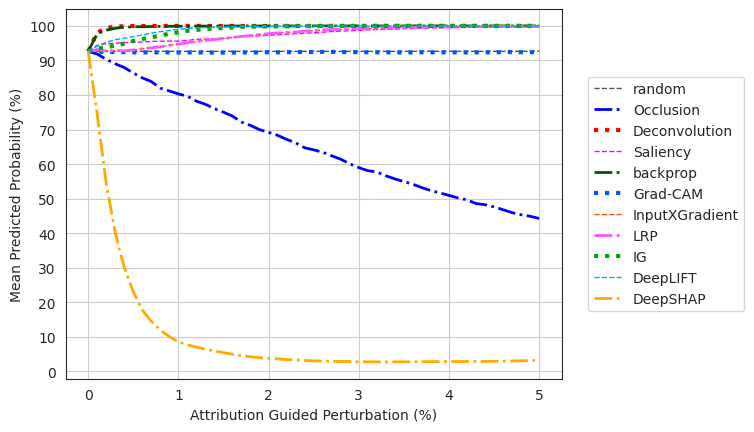
\includegraphics[width=0.8\textwidth]{figures/3672-ad-fidelity-null.png}
	\end{figure}
\end{frame}

\begin{frame}{AD to CN Perturbation: Using AD mean as Baseline}
	\begin{figure}
		\centering
		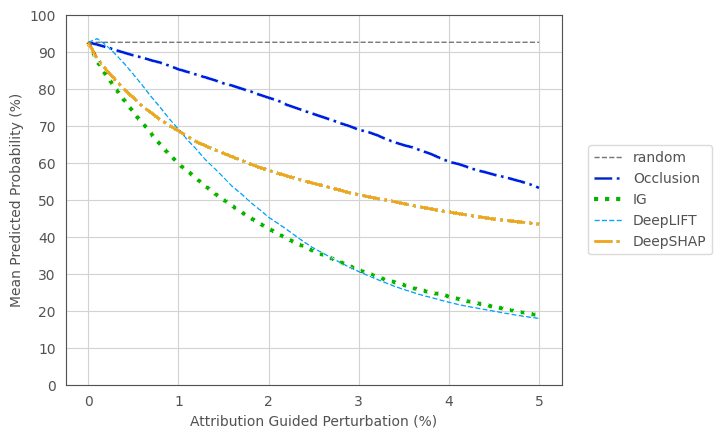
\includegraphics[width=0.8\textwidth]{figures/3672-ad-fidelity-cn2.png}
	\end{figure}
\end{frame}

% \begin{frame}{AD to CN Perturbation: Using a CN Mean as Baseline}
% 	\centering
% 	\begin{columns}
% 		\begin{column}{0.5\textwidth}
% 			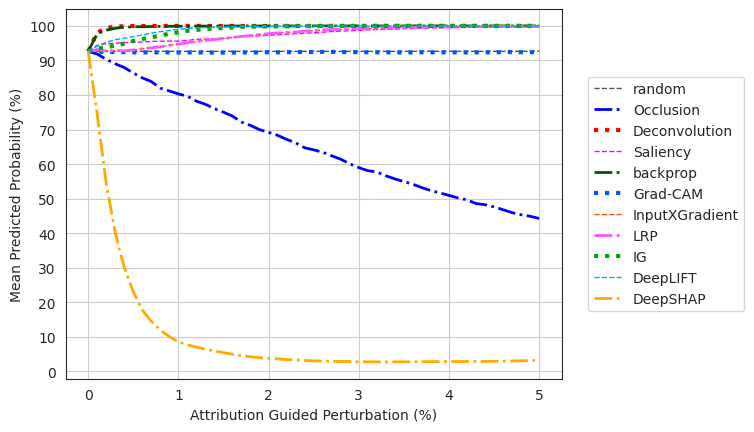
\includegraphics[width=\textwidth]{figures/3672-ad-fidelity-null.png}
% 		\end{column}\hfill
% 		\visible<2->{
% 			\begin{column}{0.5\textwidth}
% 
% 				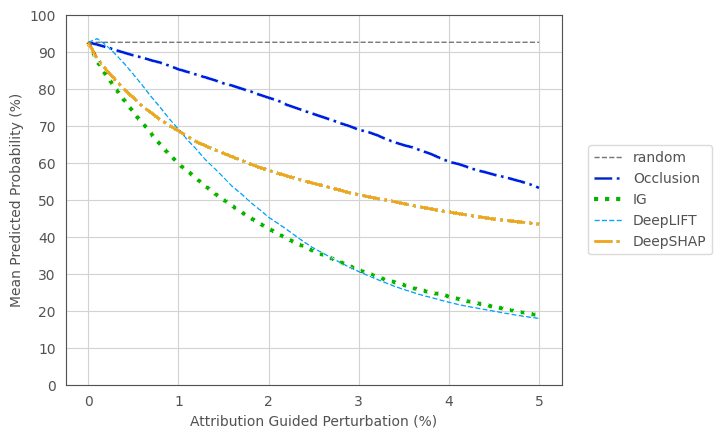
\includegraphics[width=\textwidth]{figures/3672-ad-fidelity-cn2.png}
% 			\end{column}
% 		}
% 	\end{columns}
% \end{frame}


\begin{frame}{Conclusion}
	\begin{columns}
		\begin{column}{0.5\textwidth}
			\begin{figure}
				\centering
				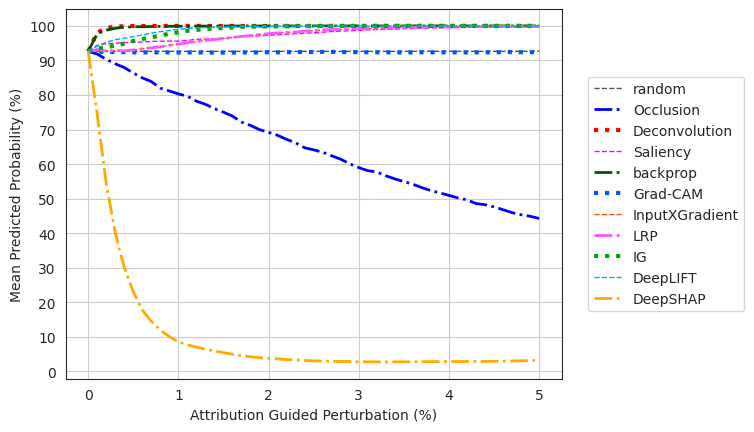
\includegraphics[width=0.8\textwidth]{figures/3672-ad-fidelity-null.png}
			\end{figure}
		\end{column}\hfill
		\begin{column}{0.5\textwidth}
			\begin{figure}
				\centering
				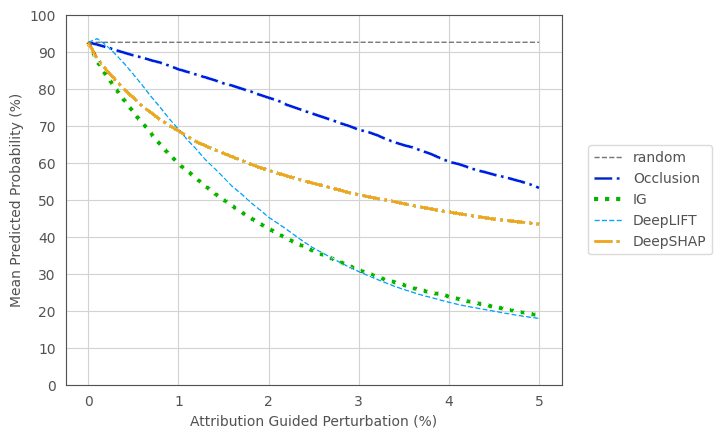
\includegraphics[width=0.8\textwidth]{figures/3672-ad-fidelity-cn2.png}
			\end{figure}
		\end{column}
	\end{columns}
	\begin{block}{Take-Aways}
		\begin{enumerate}
			\item<2-> Perturbation tests offer a \emph{model-agnostic fidelity metric}.
			\item<3-> The \emph{attribution baseline} should be chosen carefully to answer question.
			\item<4-> Attribution Maps \emph{need interpretation} to actually explain anything.
		\end{enumerate}
	\end{block}

	\visible<5->{
	}
\end{frame}

\begin{frame}{Meet the Team}
	\centering
	%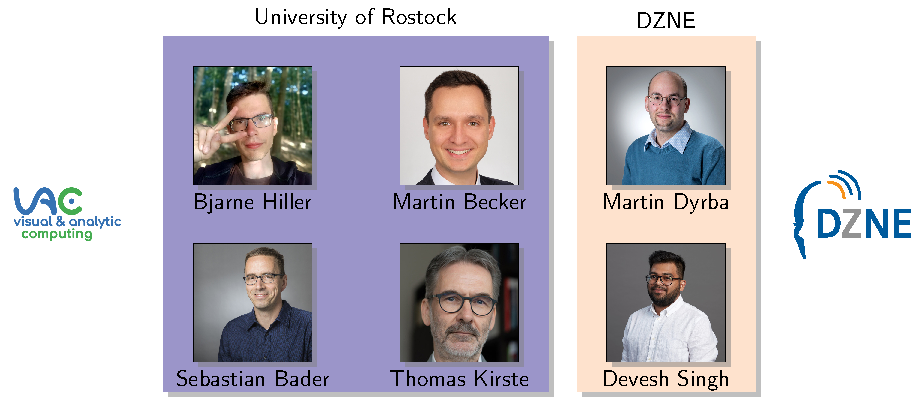
\includegraphics[width=\textwidth]{tikz/standalone/team.tikz/team.pdf}
	\resizebox{\textwidth}{!}{
		\documentclass[class=beamer, xcolor=dvipsnames, hyperref=hidelinks, preview]{standalone}

%\usepackage[dvipsnames]{xcolor}
%\usepackage[hidelinks]{hyperref}
\usepackage{tikz}
\usetikzlibrary{fit, backgrounds, positioning, shadows, shadows.blur}


\begin{document}
\tikzset{portrait/.style={draw, inner sep=0, drop shadow, on grid}}

\begin{tikzpicture}[node distance=3cm and 3.5cm]
	\node[portrait, label=below:Thomas Kirste] (kirste) {
		\href{https://www.mmis.informatik.uni-rostock.de/}{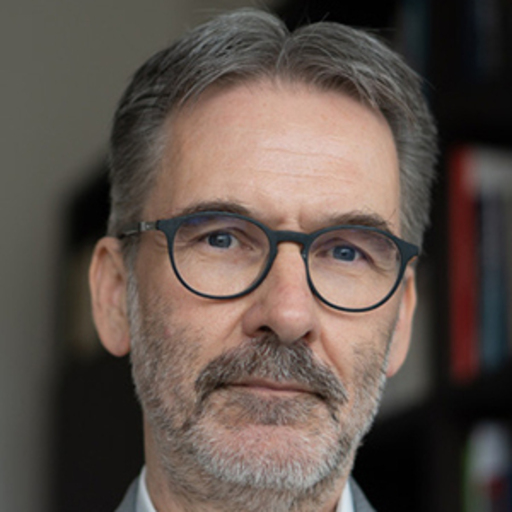
\includegraphics[width=2cm]{figures/team/thomas-kirste.jpg}}};

	\node[portrait, label=below:Sebastian Bader, below=of kirste] (bader) {
		\href{https://www.mmis.informatik.uni-rostock.de/}{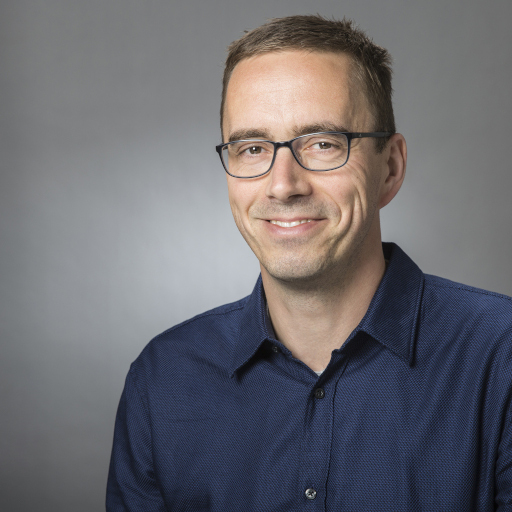
\includegraphics[width=2cm]{figures/team/sebastian-bader.jpg}}
	};

	\node[portrait, label=below:Martin Becker, right=of kirste] (becker) {
		\href{https://bckrlab.org}{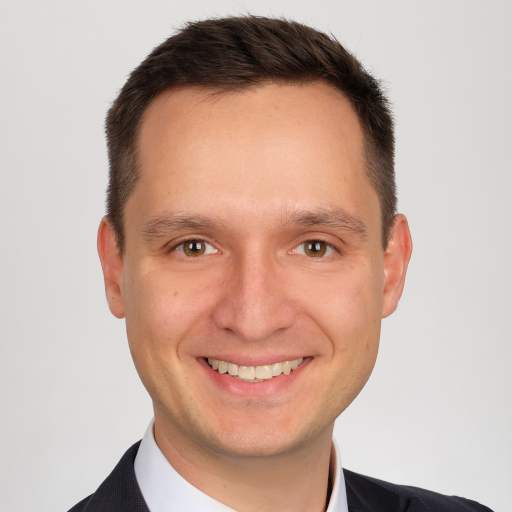
\includegraphics[width=2cm]{figures/team/martin-becker.jpg}}
	};

	\node[portrait, label=below:Bjarne Hiller, below=of becker] (hiller) {
		\href{https://github.com/chillerb}{
\includegraphics[width=2cm]{figures/team/bjarne-hiller.jpg}}
	};

	\begin{scope}[on background layer]
		\node[fit=(hiller)(kirste), rectangle, fill=Blue!40, inner sep=0.5cm, drop shadow, label=above:University of Rostock] (vac) {};
	\end{scope}

	\node[portrait, label=below:Martin Dyrba, right=of becker] (dyrba) {
		\href{https://explaination.net/}{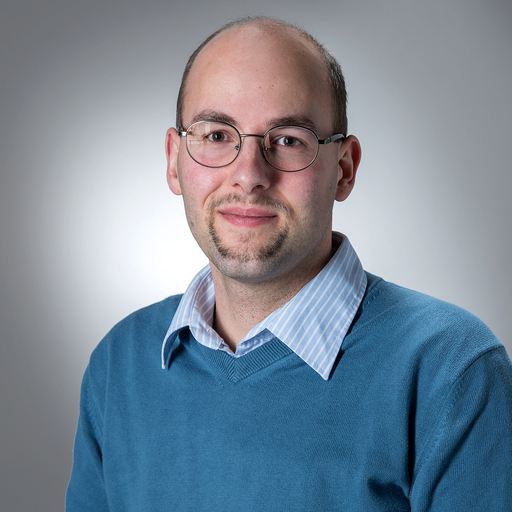
\includegraphics[width=2cm]{figures/team/martin-dyrba.jpg}}
	};

	\node[portrait, label=below:Devesh Singh, below=of dyrba] (singh) {
		\href{https://www.linkedin.com/in/deveshsingh0016/}{
\includegraphics[width=2cm]{figures/team/devesh-singh.jpg}}
	};

	\begin{scope}[on background layer]
		\node[fit=(dyrba)(singh), fill=Orange!20, rectangle, inner sep=0.5cm, drop shadow, label=above:DZNE] (dzne) {};
	\end{scope}

	% left=0.5cm of vac.west
	\node[on grid, inner sep=0, left=of kirste] {
		\href{https://vac.uni-rostock.de/}{
\includegraphics[width=2cm]{logos/logo-vac}}
	};

	% right=0.5cm of dzne.est
	\node[on grid, inner sep=0, right=of dyrba] {
		\href{https://www.dzne.de/}{
\includegraphics[width=2cm]{logos/logo-dzne}}
	};



\end{tikzpicture}
\end{document}
	}
\end{frame}

\begin{frame}{Thanks for your Attention!}
	\begin{columns}
		\begin{column}{0.5\textwidth}
			\huge
			\emph{See you on GitHub!}
			\href{https://github.com/bckrlab/ad-fidelity}{bckrlab/ad-fidelity}
		\end{column}\hfill
		\begin{column}{0.5\textwidth}
			\begin{figure}
				\href{https://github.com/bckrlab/ad-fidelity}{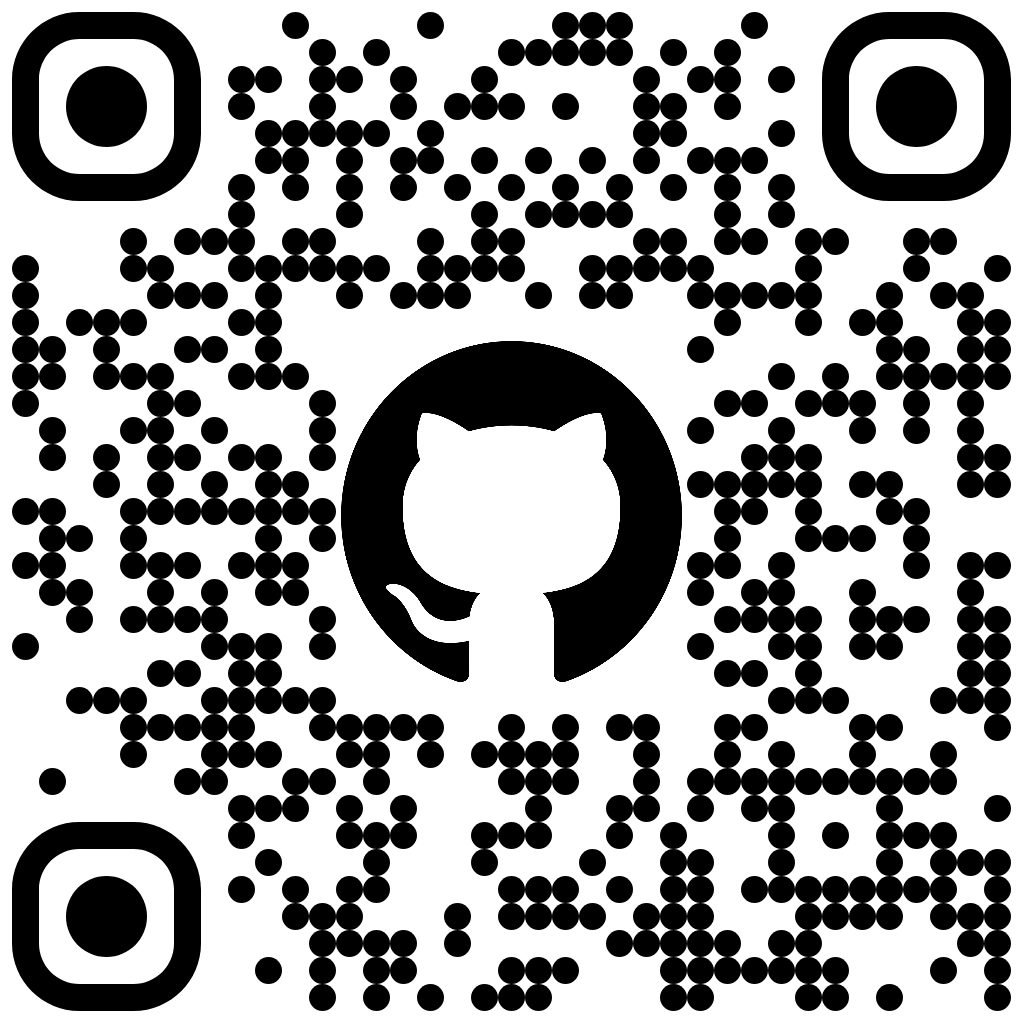
\includegraphics[width=0.9\textwidth]{figures/github-qr.png}}
			\end{figure}
		\end{column}
	\end{columns}
\end{frame}

\begin{frame}[allowframebreaks]{References}
	\tiny
	\printbibliography[heading=none]
\end{frame}

\end{document}